% Misc. Definitions
%% Color definitions
\definecolor{Fgreen}{RGB}{34,139,34}


%--------------------------------------------------
% Introduction
%--------------------------------------------------
%--------------------------------------------------

DEFINE BASE PROBLEM, AND DISCUSS WHAT WE MEAN BY "LOCAL MEASUREMENTS"!!!\\

%Angular synchronization refers to the problem of recovering $d$ angles
%$\phi_1, \phi_2, \dots, \phi_d \in [0, 2\pi)$ given noisy and possibly
%    incomplete difference measurements of the form
%%
%\[  \phi_{ij} := \phi_i - \phi_j, \qquad (i,j) \in 
%        \{1,2,\dots,d\} \times \{1,2,\ldots,d\}. \]
%%
%This problem has important applications in network delay analysis
%\cite{network_ref}, optics \cite{optics_ref} and computer vision
%\cite{cvision_ref}. In this paper, however, we are interested in angular
%synchronization problems that arise when performing {\em phase
%retrieval} from {\em local correlation} measurements. 
The phase
retrieval problem \cite{balan2006signal,shechtman2015phase} is seen, for example, in
molecular imaging modalities such as X-Ray crystallography and
Ptychography \cite{Rodenburg2008}, where the underlying physics dictates
that we can only acquire (squared) magnitude or phaseless measurements.
As one may imagine, this is an extremely challenging
mathematical problem even in the setting when the measurements are noise-free as the phase encapsulates a significant amount of
structure in the underlying signal. %hence, recovering the signal from phaseless data is a non-trivial task. 
To complicate things further, often the physics associated with the problem constrains the type of measurements one acquires. For example, in ptychographic
imaging, the imaging system acquires a sequence of possibly noisy, {\em local} (as
opposed to {\em global}) snapshots of the magnitude of the underlying specimen. %The need
%to minimize the number of measurements acquired and inevitable
%measurement errors in the imaging process only accentuate the complexity
%of this phase retrieval problem.

%
\begin{figure}[hbtp]
    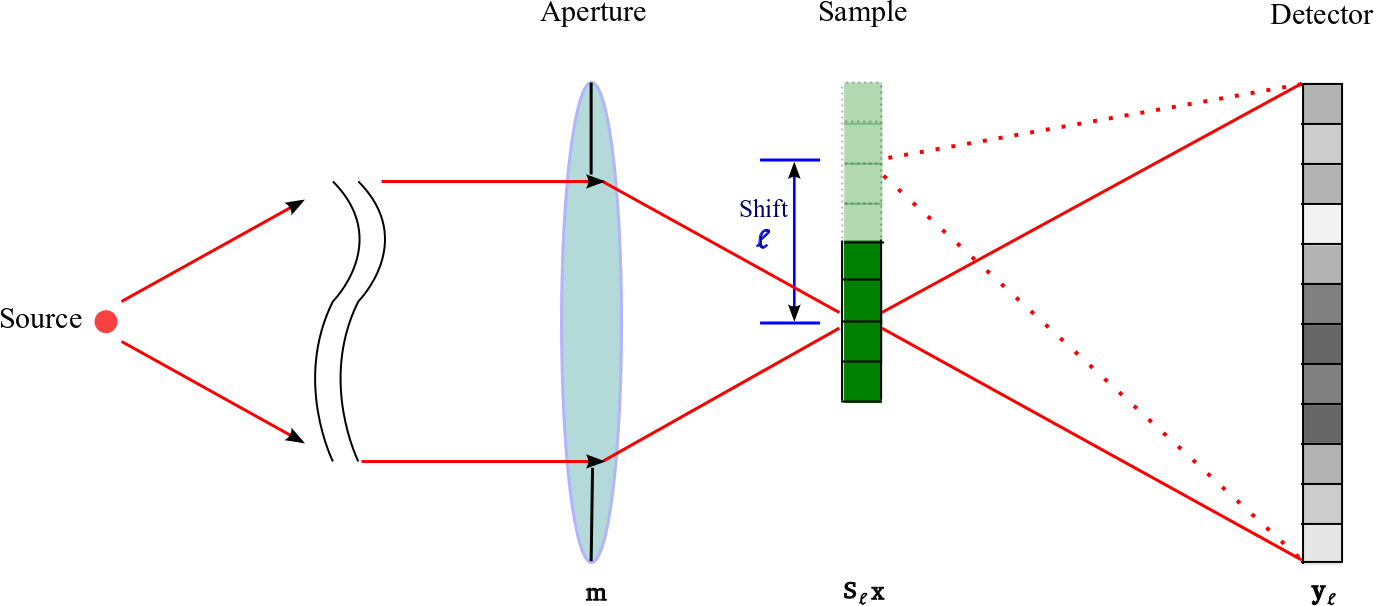
\includegraphics[scale=0.25]{pics/ptych1D}
    \caption{Illustration of Ptychographic Imaging {\small 
        (Adapted from ``Fly-scan ptychography'', Huang et al., 
        Scientific Reports 5 (9074), 2015.)} }
    \label{fig:ptychography_setup}
\end{figure}
%
To set the stage for the discussion in this paper, consider the
one-dimensional ptychographic imaging setup in Fig.
\ref{fig:ptychography_setup}, where an intensity\footnote{By intensity, we mean magnitude squared.} detector captures the
far-field diffraction pattern resulting from irradiating a small region
of the test sample. Under certain conditions (appropriate wavelength of
incident radiation, far-field Fresnel approximation), it is possible to
show that the acquired magnitude measurements are in fact Fourier
measurements of the form 
%
\begin{equation*}
    y_\ell = \left \vert \mathcal F [ \widetilde m \circ S_\ell x ]
       \right \vert^2,
\end{equation*}
%
where $\mathcal F$ denotes the Fourier transform, $x$ is the unknown
test specimen, $S_\ell x$ is a shift or translation of $x$; i.e.,
$(S_\ell x)(j) := x(j+\ell)$, $\widetilde m$ is the aperture
transmission function of the imaging system, and $\circ$ denotes elementwise multiplication (see, for example, \cite{}){\color{red} We need some citations here}. %Note that squaring the magnitude of the Fourier transform above means that $y_\ell$ is a
%phaseless diffraction measurement corresponding to a specific shift (by
%$\ell$) of the test specimen.  
Moreover, we assume that $\text{supp}(\widetilde m) \subset \text{supp} (x)$, so $y_\ell$ is a  {\em local} phaseless diffraction
measurement. % corresponding to a shift by $\ell$ of the test specimen. 
 The imaging process involves acquiring a sequence of such measurements
corresponding to several $\ell$-shifts of the sample. In the discrete setting, this becomes\footnote{We use the notation $(\x)_k$ to denote the
$k^{th}$ entry of the vector $\x$.} 
%
\begin{equation}
    (\y_\ell)_j = \left \vert \sum_{n=1}^d \widetilde m_n \, x_{n+\ell-1} \,
      \mathbbm e^{-\frac{2\pi \mathbbm i (j-1) (n-1)}d} 
      \right \vert^2, \quad (j,\ell) \in \{1,2,\dots,d\} \times  
      \{0,1,2,\dots,d-1\}, 
  \label{eq:1d_ptycho}
\end{equation}
%
where $\x, \widetilde \m \in \mathbbm C^d$ and all indexing is
considered modulo-$d$. As in the continuous formulation, $(\y_\ell)_j$
is a diffraction measurement corresponding to the $j^{th}$ Fourier mode
and a circular $\ell$-shift of the specimen. In addition, since
$\widetilde \m$ represents a {\em local} image snapshot, we assume that
$\widetilde m_j = 0$ for $j>\delta \in \mathbbm N$. In this paper, we
will work with the following more convenient form of (\ref{eq:1d_ptycho}):
%
\begin{equation}
    (\y_\ell)_j = \left \vert \sum_{n=1}^d x_{n+\ell-1} \, \left( \widetilde 
        m_n \, \mathbbm e^{-\frac{2\pi \mathbbm i (j-1) (n-1)}d} 
        \right) \right \vert^2 := 
        \left \vert \sum_{n=1}^d x_{n+\ell-1} \, (\m_j)_n \right \vert^2 = 
        \left \vert \sum_{n=1}^\delta x_{n+\ell-1} \, (\m_j)_n \right \vert^2 
  \label{eq:loco_measurements}
\end{equation}
%
where the local support of $\m_j \in \mathbbm C^d$ follows from the
locality of $\widetilde \m$. We note that (\ref{eq:loco_measurements})
defines a {\em correlation} with {\em local} masks or window functions
$\m_j$. To see how an angular synchronization problem manifests in the
course of solving this phase retrieval problem, consider a simple but
illustrative example of recovering an unknown vector $\x \in \mathbbm
C^4$ from noiseless measurements
%
\[ \y = \left \vert M \x \right \vert^2, \]
%
where $\y \in \mathbbm R^{12}$ and $M \in \mathbbm C^{12\times 4}$.
Since we consider local correlation measurements, $M$ is
block-circulant with the following structure: 
%
\[ M =  \begin{bmatrix}
            M_1 \\ M_2 \\ M_3 
        \end{bmatrix}, \quad 
    M_i =   \begin{bmatrix}
                (\m_i)_1 & (\m_i)_2 & 0 & 0 \\
                0 & (\m_i)_1 & (\m_i)_2 & 0 \\
                0 & 0 & (\m_i)_1 & (\m_i)_2 \\
                (\m_i)_2 & 0 & 0 & (\m_i)_1 
            \end{bmatrix}.       \]
%
Here, the masks $\m_{\{1,2,3\}} \in \mathbbm C^4$ have local support
with $(\m_{\{1,2,3\}})_j = 0$ for $j=3,4$. This setup corresponds to
local correlation measurements of the form
%
\begin{equation*}
    \left( \y_\ell \right)_i = 
    \left \vert \sum_{k=1}^{\delta=2}
        ({\bf m_i})_k \cdot x_{\ell+k-1} \right \vert^2, 
        \qquad (\ell, i) \in \{1,2,3\} \times \{1,2,3,4\}.
\end{equation*}
%
Expanding the squared correlation sum, we obtain
%
\begin{equation*}
    \left( \y_\ell \right)_i = 
        \left \vert \sum_{k=1}^\delta 
            ({\bf m_i})_k \cdot x_{\ell+k-1} 
            \right \vert^2 
        = \sum_{j,k=1}^\delta ({\bf m_i})_j \, ({\bf m_i})_k^* \, 
        x_{\ell+j-1} \, x_{\ell+k-1}^* 
       := \sum_{j,k=1}^\delta ({\bf m_i})_{j,k} \,
            x_{\ell+j-1} \, x_{\ell+k-1}^*,
\end{equation*}
%
Since the masks $\m_{\{1,2,3\}}$ (which are related to the aperture
transmission function of the imaging system) are known - either by design or
through calibration, the above equation describes a linear system of equations
for the $D=(2\delta-1)d=12$ (scaled) local phase differences $\left \lbrace
x_ix_j^* \right \rbrace_{|i-j\mod \; 4| = 1}$. Specifically, we have the 
system $M^\prime \z = \widetilde \b$, where 
%
\[  {\bf z} =  
\begin{bmatrix}
    |x_1|^2 & x_1x_2^* & 
    x_2x_1^* & |x_2|^2 & x_2x_3^* & 
    x_3x_2^* & |x_3|^2 & x_3x_4^* &
    x_4x_3^* & |x_4|^2 & x_4x_1^* & x_1x_4^*
\end{bmatrix}^T   \]
%
is a vector of scaled local phase differences,
%
\[  \widetilde \b = 
\begin{bmatrix}
    (\y_1)_1 & (\y_2)_1 & (\y_3)_1 & 
    (\y_1)_2 & (\y_2)_2 & (\y_3)_2 & 
    (\y_1)_3 & (\y_2)_3 & (\y_3)_3 &
    (\y_1)_4 & (\y_2)_4 & (\y_3)_4
\end{bmatrix}^T      \]
%
is an interleaved vector of measurements (obtained by permuting the entries
of $\y$), and 
%
\[ 
  \arraycolsep=1.4pt\def\arraystretch{0.3}
  \! \! M^\prime \! \! \! = \! \! \!
    \left(  \! \! 
    \begin{array}{ccc;{2pt/2pt}ccc;{2pt/2pt}ccc;{2pt/2pt}ccc}
        \textcolor{red}{({\bf m}_1)_{\mbox{\tiny 1,1}}} & 
        \textcolor{red}{({\bf m_1})_{\mbox{\tiny 1,2}}} & 
        \textcolor{red}{({\bf m}_1)_{\mbox{\tiny 2,1}}} & 
        \textcolor{blue}{({\bf m}_1)_{\mbox{\tiny 2,2}}} & 
        \textcolor{blue}{0} & 
        \textcolor{blue}{0} & 
        0 & 0 & 0 & 0 & 0 & 0\\
        \textcolor{red}{({\bf m}_2)_{\mbox{\tiny 1,1}}} & 
        \textcolor{red}{({\bf m}_2)_{\mbox{\tiny 1,2}}} & 
        \textcolor{red}{({\bf m}_2)_{\mbox{\tiny 2,1}}} & 
        \textcolor{blue}{({\bf m}_2)_{\mbox{\tiny 2,2}}} & 
        \textcolor{blue}{0} & \textcolor{blue}{0} & 0 & 0 & 0 & 0 & 0 & 0\\
        \textcolor{red}{({\bf m}_3)_{\mbox{\tiny 1,1}}} & 
        \textcolor{red}{({\bf m}_3)_{\mbox{\tiny 1,2}}} & 
        \textcolor{red}{({\bf m}_3)_{\mbox{\tiny 2,1}}} & 
        \textcolor{blue}{({\bf m}_3)_{\mbox{\tiny 2,2}}} & 
        \textcolor{blue}{0} & \textcolor{blue}{0} & 0 & 0 & 0 & 0 & 0 & 0
        \vspace{0.05in} \\ \hdashline[2pt/2pt]
        & & & \vspace{-0.02in} \\
        0 & 0 & 0 & 
        \textcolor{red}{({\bf m}_1)_{\mbox{\tiny 1,1}}} & 
        \textcolor{red}{({\bf m_1})_{\mbox{\tiny 1,2}}} & 
        \textcolor{red}{({\bf m}_1)_{\mbox{\tiny 2,1}}} & 
        \textcolor{blue}{({\bf m}_1)_{\mbox{\tiny 2,2}}} & 
        \textcolor{blue}{0} & \textcolor{blue}{0} & 0 & 0 & 0\\
        0 & 0 & 0 & 
        \textcolor{red}{({\bf m}_2)_{\mbox{\tiny 1,1}}} & 
        \textcolor{red}{({\bf m}_2)_{\mbox{\tiny 1,2}}} & 
        \textcolor{red}{({\bf m}_2)_{\mbox{\tiny 2,1}}} & 
        \textcolor{blue}{({\bf m}_2)_{\mbox{\tiny 2,2}}} & 
        \textcolor{blue}{0} & \textcolor{blue}{0} & 0 & 0 & 0\\
        0 & 0 & 0 & 
        \textcolor{red}{({\bf m}_3)_{\mbox{\tiny 1,1}}} & 
        \textcolor{red}{({\bf m}_3)_{\mbox{\tiny 1,2}}} & 
        \textcolor{red}{({\bf m}_3)_{\mbox{\tiny 2,1}}} & 
        \textcolor{blue}{({\bf m}_3)_{\mbox{\tiny 2,2}}} & 
        \textcolor{blue}{0} & \textcolor{blue}{0} & 0 & 0 & 0
        \vspace{0.05in} \\ \hdashline[2pt/2pt]
        & & & \vspace{-0.02in} \\
        0 & 0 & 0 & 0 & 0 & 0 & 
        \textcolor{red}{({\bf m}_1)_{\mbox{\tiny 1,1}}} & 
        \textcolor{red}{({\bf m_1})_{\mbox{\tiny 1,2}}} & 
        \textcolor{red}{({\bf m}_1)_{\mbox{\tiny 2,1}}} & 
        \textcolor{blue}{({\bf m}_1)_{\mbox{\tiny 2,2}}} & 
        \textcolor{blue}{0} & \textcolor{blue}{0} \\
        0 & 0 & 0 & 0 & 0 & 0 & 
        \textcolor{red}{({\bf m}_2)_{\mbox{\tiny 1,1}}} & 
        \textcolor{red}{({\bf m}_2)_{\mbox{\tiny 1,2}}} & 
        \textcolor{red}{({\bf m}_2)_{\mbox{\tiny 2,1}}} & 
        \textcolor{blue}{({\bf m}_2)_{\mbox{\tiny 2,2}}} & 
        \textcolor{blue}{0} & \textcolor{blue}{0} \\
        0 & 0 & 0 & 0 & 0 & 0 & 
        \textcolor{red}{({\bf m}_3)_{\mbox{\tiny 1,1}}} & 
        \textcolor{red}{({\bf m}_3)_{\mbox{\tiny 1,2}}} & 
        \textcolor{red}{({\bf m}_3)_{\mbox{\tiny 2,1}}} & 
        \textcolor{blue}{({\bf m}_3)_{\mbox{\tiny 2,2}}} & 
        \textcolor{blue}{0} & \textcolor{blue}{0}
        \vspace{0.05in} \\ \hdashline[2pt/2pt]
        & & & \vspace{-0.02in} \\
        \textcolor{blue}{({\bf m}_1)_{\mbox{\tiny 2,2}}} & 
        \textcolor{blue}{0} & \textcolor{blue}{0} & 0 & 0 & 0 & 0 & 0 & 0 & 
        \textcolor{red}{({\bf m}_1)_{\mbox{\tiny 1,1}}} & 
        \textcolor{red}{({\bf m_1})_{\mbox{\tiny 1,2}}} & 
        \textcolor{red}{({\bf m_1})_{\mbox{\tiny 2,1}}} \\
        \textcolor{blue}{({\bf m}_2)_{\mbox{\tiny 2,2}}} & 
        \textcolor{blue}{0} & \textcolor{blue}{0} & 0 & 0 & 0 & 0 & 0 & 0 & 
        \textcolor{red}{({\bf m}_2)_{\mbox{\tiny 1,1}}} & 
        \textcolor{red}{({\bf m_2})_{\mbox{\tiny 1,2}}} & 
        \textcolor{red}{({\bf m_2})_{\mbox{\tiny 2,1}}} \\
        \textcolor{blue}{({\bf m}_3)_{\mbox{\tiny 2,2}}} & 
        \textcolor{blue}{0} & \textcolor{blue}{0} & 0 & 0 & 0 & 0 & 0 & 0 & 
        \textcolor{red}{({\bf m}_3)_{\mbox{\tiny 1,1}}} & 
        \textcolor{red}{({\bf m_3})_{\mbox{\tiny 1,2}}} & 
        \textcolor{red}{({\bf m_3})_{\mbox{\tiny 2,1}}}
    \end{array}  \! \!   \right) \! \!.    \] 
%
Clearly, $M^\prime$ is composed of two blocks $M_1^\prime,M_2^\prime\in
\mathbbm C^{3 \times 3}$ highlighted using dashed lines. We can show
(see \cite{IVW2015_FastPhase} for details and Section \ref{sec:fastloco} for
a summary of the results) that $M^\prime$ is well-conditioned for
suitable choise of masks $\m$. Moreover, $M^\prime$ can be efficiently
inverted in FFT-time to obtain the scaled phase differences
$\{x_ix_j^*\}$.


We now show that the process of recovering $\x$ from $\{x_ix_j^*\}$
is equivalent to solving an angular synchronization problem.  We begin
by noting that the vector $\z$ in our example problem above indexes the
$(2\delta-1)$ entries on the rows of the rank-1 matrix $\x \x^*$. Hence,
re-arranging 
%
\[    
\begin{bmatrix}
    \textcolor{red}{|x_1|^2} ~
    \textcolor{red}{x_1x_2^*} ~ 
    \textcolor{blue}{x_2x^*_1} ~ 
    \textcolor{blue}{|x_2|^2} ~ 
    \textcolor{blue}{x_2x_3^*} ~ 
    \textcolor{Fgreen}{x_3x^*_2} ~
    \textcolor{Fgreen}{|x_3|^2} ~ 
    \textcolor{Fgreen}{x_3x_4^*} ~ 
    \textcolor{black}{x_4x^*_3} ~
    \textcolor{black}{|x_4|^2} ~ 
    \textcolor{black}{x_4x_1^*} ~ 
    \textcolor{red}{x_1x^*_4}
\end{bmatrix}^T,    \]
%
we obtain
%
\[ X_0 = \begin{bmatrix}
    & \textcolor{red}{|x_1|^2} & &
    \textcolor{red}{x_1x_2^*} & & 
    0 & &
    \textcolor{red}{x_1x^*_4} & \\
    & 
    \textcolor{blue}{x_2x^*_1} & &
    \textcolor{blue}{|x_2|^2} & &
    \textcolor{blue}{x_2x_3^*} & &
    0 & \\
    & 0 & & 
    \textcolor{Fgreen}{x_3x^*_2} & &
    \textcolor{Fgreen}{|x_3|^2} & &
    \textcolor{Fgreen}{x_3x_4^*} & & \\
    & \textcolor{black}{x_4x_1^*} & &
    0 &  &
    \textcolor{black}{x_4x^*_3} & &
    \textcolor{black}{|x_4|^2} &
\end{bmatrix}.      \]
%
Observe that the magnitudes of $\x$ can now be obtained from the main
diagonal of $X_0$. In addition, if we normalize each entry of this
matrix by its magnitude, we obtain 
%
\[  \widetilde X_0 = \begin{bmatrix}
    \textcolor{red}{1} & 
    \textcolor{red}{e^{\mathbbm i (\phi_1 - \phi_2)}} & 
    0 &
    \textcolor{red}{e^{\mathbbm i (\phi_1 - \phi_4)}} \\
    \textcolor{blue}{e^{\mathbbm i (\phi_2 - \phi_1)}} & 
    \textcolor{blue}{1} & 
    \textcolor{blue}{e^{\mathbbm i (\phi_2 - \phi_3)}} & 
    0 \\
    0 & 
    \textcolor{Fgreen}{e^{\mathbbm i (\phi_3 - \phi_2)}} & 
    \textcolor{Fgreen}{1} & 
    \textcolor{Fgreen}{e^{\mathbbm i (\phi_3 - \phi_4)}} \\
    \textcolor{black}{e^{\mathbbm i (\phi_4 - \phi_1)}} & 
    0 &
    \textcolor{black}{e^{\mathbbm i (\phi_4 - \phi_3)}} & 
    \textcolor{black}{1} & 
\end{bmatrix}.       \] 
%
We note that the phase angle of the $(i,j)^{th}$ entry of $\widetilde
X_0$ is the difference in phase angle between components $x_i$ and $x_j$
of our unknown vector $\x$. Moreover, we have such phase difference data
spanning each component $x_i$ and its $\delta$ neighbors. This
neighborhood arises directly from the local nature of our measurements.
We can solve this angular synchronization problem by computing the
leading eigenvector. For our example problem, it is easy to see that 
%
\[  \begin{bmatrix}
    \textcolor{red}{1} & 
    \textcolor{red}{e^{\mathbbm i (\phi_1 - \phi_2)}} & 
    0 &
    \textcolor{red}{e^{\mathbbm i (\phi_1 - \phi_4)}} \\
    \textcolor{blue}{e^{\mathbbm i (\phi_2 - \phi_1)}} & 
    \textcolor{blue}{1} & 
    \textcolor{blue}{e^{\mathbbm i (\phi_2 - \phi_3)}} & 
    0 \\
    0 & 
    \textcolor{Fgreen}{e^{\mathbbm i (\phi_3 - \phi_2)}} & 
    \textcolor{Fgreen}{1} & 
    \textcolor{Fgreen}{e^{\mathbbm i (\phi_3 - \phi_4)}} \\
    \textcolor{black}{e^{\mathbbm i (\phi_4 - \phi_1)}} & 
    0 &
    \textcolor{black}{e^{\mathbbm i (\phi_4 - \phi_3)}} & 
    \textcolor{black}{1} & 
\end{bmatrix} 
\underbrace{
    \begin{bmatrix}
        \textcolor{red}{e^{\mathbbm i \phi_1}} \\
        \textcolor{blue}{e^{\mathbbm i \phi_2}} \\
        \textcolor{Fgreen}{e^{\mathbbm i \phi_3}} \\
        \textcolor{black}{e^{\mathbbm i \phi_4}}
    \end{bmatrix}   }_{\text{leading eigenvector}} = 
    \underbrace{3}_{2\delta-1}
\underbrace{
    \begin{bmatrix}
        \textcolor{red}{e^{\mathbbm i \phi_1}} \\
        \textcolor{blue}{e^{\mathbbm i \phi_2}} \\
        \textcolor{Fgreen}{e^{\mathbbm i \phi_3}} \\
        \textcolor{black}{e^{\mathbbm i \phi_4}}
    \end{bmatrix}   }_{\text{leading eigenvector} = \angle \x },
\] 
%
with the final reconstruction given by
%
\[
    \begin{bmatrix}
      \textcolor{red}{|x_1|} e^{\mathbbm i \, 
            \textcolor{red}{\phi_1}} & 
      \textcolor{blue}{|x_2|} e^{\mathbbm i \, 
            \textcolor{blue}{\phi_2}} & 
      \textcolor{Fgreen}{|x_3|} e^{\mathbbm i \, 
            \textcolor{Fgreen}{\phi_3}} & 
      \textcolor{black}{|x_4|} e^{\mathbbm i \, 
            \textcolor{black}{\phi_4}}
    \end{bmatrix}^T.    \]
%
In \cite{IV_SPIE}, it was shown that the phase of the $\x$ is
indeed given by the leading eigenvector of $\widetilde X_0$. Moreover,
it was shown that this eigenvector is unique and corresponds to an
eigenvalue of $2\delta-1$. The perturbation theory for this eigenvector
method and associated recovery guarantees for the phase retrieval
problem are the subject of this paper. 
%
%
%--------------------------------------------------
% Main Result 
%--------------------------------------------------
\subsection{Main Result}
\label{sec:mainRes}
Include main theorem(s) here!!!
%
%%%
%
%--------------------------------------------------
% Literature Survey 
%--------------------------------------------------
\subsection{Related Work}
\label{sec:lit}

-- early mathy phase retrieval papers \cite{balan2006signal,balan2009painless}.\\

--Alternating projection techniques \cite{gerchberg1972practical,fienup1978reconstruction} work well in practice and have been popular for decades, but are notoriously difficult to analyze.  These iterative methods work by improving an initial guess until they stagnate.  Recently Marchesini et al. proved that alternating projection schemes using generic measurements are guaranteed to converge to the correct solution {\em if provided with a sufficiently accurate initial guess}, and algorithms for ptychography were explored in particular \cite{marchesini2015alternating}.  However, no global recovery guarantees currently exist for alternating projection techniques utilizing local measurements (i.e., finding a sufficiently accurate initial guess is not generally easy).\\

-- probabilistic recovery guarantees have been proven for many methods when provided with global gaussian measurements, including: methods based on convex optimization techniques \cite{candes2012phaselift,candes2014solving}, methods based on (stochastic) gradient decent strategies \cite{candes2015phase}, methods based on graph-theoretic and frame-based approaches  \cite{alexeev2014phase}, and alternating minimization methods variants (e.g., with resampling) \cite{netrapalli2013phase}. \\

-- Several recovery algorithms achieve theoretical recovery guarantees while using at most $D = \mathcal{O}(d \log^4 d)$ masked Fourier coded diffraction pattern measurements, including both {\em PhaseLift} \cite{Candes2014WF,gross2015improved}, and {\em Wirtinger Flow} \cite{candes2015phase}.  However, these measurements are both randomized (which is crucial to the probabilistic recovery guarantees developed for both PhaseLift and Wirtinger Flow -- deterministic recovery guarantees do not exist for either method in the noisy setting), and provide global information about $\x_0$ from each measurement (i.e., the measurements are not local).\\

-- Local measurements:  In \cite{eldar2014sparse,jaganathan2015stft} it is shown that STFT measurements with specific properties can allow (sparse) phase retrieval in the noiseless setting, and several recovery methods are proposed.  Similarly, the phase retrieval approach from \cite{alexeev2014phase} is extended to STFT measurements in \cite{salanevich2015polarization} in order to produce recovery guarantees in the noiseless setting. However, no recovery guarantees are proven in the noisy setting for any of these approaches.  Aditya and my paper \cite{IVW2015_FastPhase}...\\


-------------------------------------------------------------------------------------------

The remainder of this paper is organized as follows: Section
\ref{sec:fastloco} begins by summarizing relevant results from
\cite{IVW2015_FastPhase} concerning local
correlation measurement constructions, and then briefly introduces the new lifting-based phase retrieval approach for local measurements considered herein.  
The new recovery algorithm for local
correlation measurements is then discussed in detail in Section~\ref{sec:TheAlg}, and it is shown in Section~\ref{sec:STFT} that the same approach can also be 
used to solve the problem of phase retrieval from Short Time Fourier Transform (STFT) magnitude measurements. In Section~\ref{sec:Spectrum}, we begin
our analysis of the proposed phrase retrieval method by discussing the
spectrum of matrices like $\widetilde X_0$ above, while Section~\ref{sec:Perturb} develops perturbation results concerning their top eigenvectors.  Recovery guarantees for the proposed phase
retrieval method are then developed in Section~\ref{sec:RecovGuarantee}. Numerical results verifying the accuracy,
efficiency, and robustness of the proposed methods are finally provided in
Section \ref{sec:NumEval}, while Section \ref{sec:conclusion} contains
some concluding remarks and avenues for further research.

